
\documentclass[twoside,onecolumn]{article}

\usepackage{blindtext} % Package to generate dummy text throughout this template 

%\usepackage[sc]{mathpazo} % Use the Palatino font
\usepackage[T1]{fontenc} % Use 8-bit encoding that has 256 glyphs
\linespread{1.05} % Line spacing - Palatino needs more space between lines
\usepackage{microtype} % Slightly tweak font spacing for aesthetics
\usepackage{float}
 \usepackage{amsmath}
 \usepackage{booktabs}
 \usepackage{amssymb}
 \usepackage{amsthm}
 \usepackage{tabularx} %tabelle
 \usepackage{tikz} %circuiti
 \usepackage{enumerate}
 \usepackage{pgfplots}
 \usepackage{subcaption}
\usepackage[toc,page]{appendix}
 \usepackage[export]{adjustbox}
 \usepackage{caption}
 \usepackage{subfig}
 \usepackage{sidecap}
 \usepackage{graphicx}
 \theoremstyle{definition}
  \usepackage{multicol}
  \usetikzlibrary{arrows}
  
\usepackage[english]{babel} % Language hyphenation and typographical rules

\usepackage[hmarginratio=1:1,top=32mm,columnsep=20pt]{geometry} % Document margins
\usepackage[hang, small,labelfont=bf,up,textfont=it,up]{caption} % Custom captions under/above floats in tables or figures
\usepackage{booktabs} % Horizontal rules in tables

\usepackage{lettrine} % The lettrine is the first enlarged letter at the beginning of the text

\usepackage{enumitem} % Customized lists
\setlist[itemize]{noitemsep} % Make itemize lists more compact

\usepackage{titlesec} % Allows customization of titles
\titleformat{\section}[block]{\large\scshape\centering}{\thesection.}{1em}{} % Change the look of the section titles
\titleformat{\subsection}[block]{\large}{\thesubsection.}{1em}{} % Change the look of the section titles

\usepackage{hyperref} % For hyperlinks in the PDF

\title{Homework 1: Summarizing Performance Data } % Article title
\author{Nicole Zattarin}
\date{} 
\begin{document}

% Print the title
\maketitle

\section{Comparing data: the example of two operating systems }
\subsection{Display distributions}
Let us consider the example of two operating systems: an older one and its new version, whose performances are supposed to be better then the previous one. We aim to compare these two options by studying the execution times of a series of commonly used programs with both options. \par
In Figure \ref{fig:distribution_scatter} we report both the distributions and the individual data for each of the two versions. It is possible to highlight that the histograms provide informations regarding the statistical distributions of data, while scatterplots allow us only to individuate a qualitative trend in the observed data.  A more quantitative way to extrapolate information from the data consist of comparing the cumulative density functions of the two distributions, in Figure \ref{fig:cdf} we report the CDF for both the versions of the operating system. It is possible to observe that, since the CDF corresponding to the execution times of the new systems is almost constantly above the function of the older version, that the first provide a better alternative to the latter. Finally, it may be useful to compare two distributions is by means of boxplots, swarmplots and violinplots, in Figure \ref{fig:boxswarm} we provide both boxplots and swarmplots of each of the two distributions. Such tools are particularly useful to represent quantiles and, for what concerns violinplots and swarmplots, a qualitative shape of the distribution, as it is possible to observe in Figure \ref{fig:boxswarm}.


\begin{figure} \centering
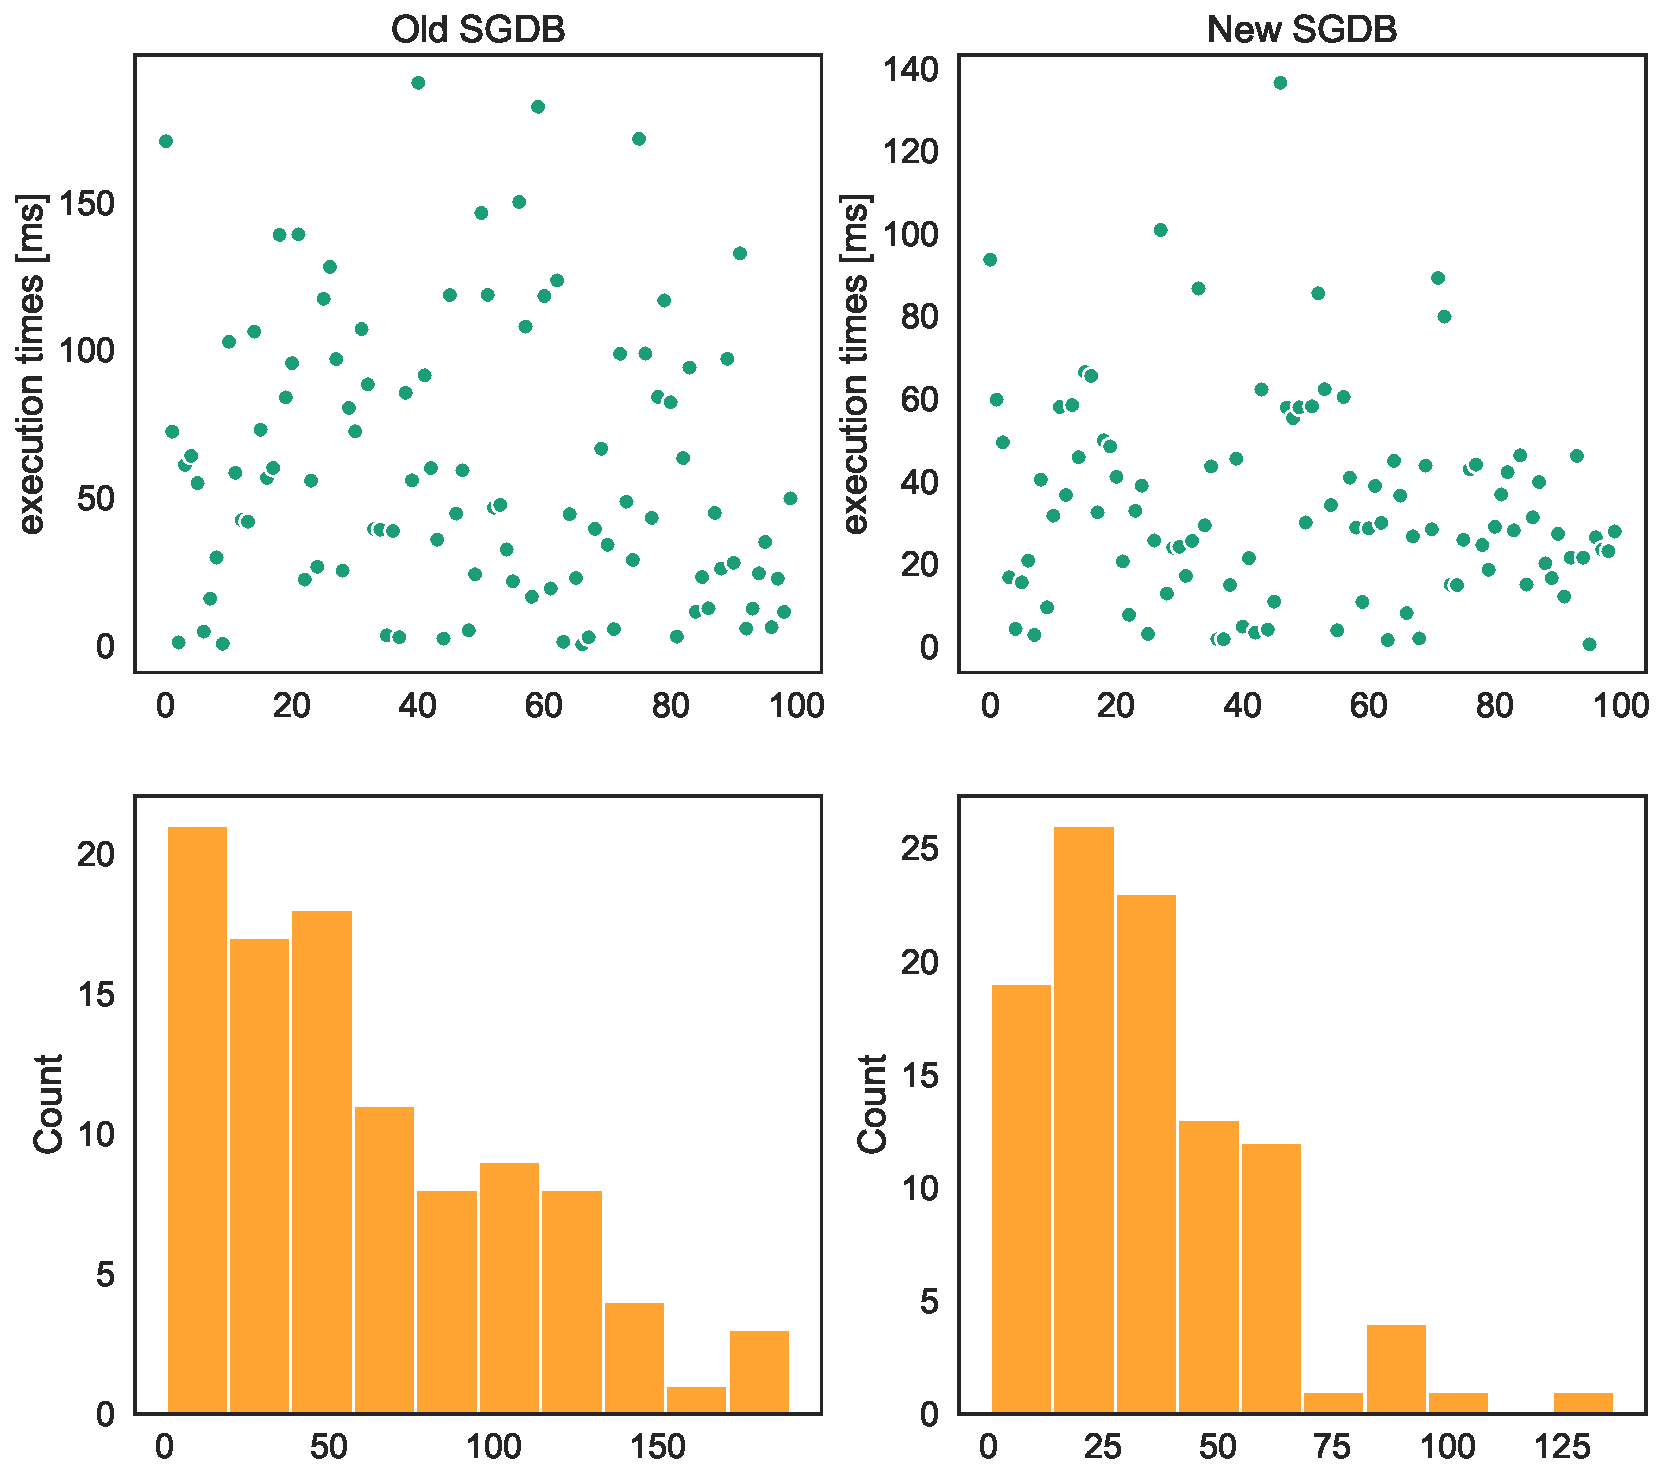
\includegraphics[width=0.8\textwidth]{../figs/extimes_distributions_vs_scatter.pdf}
\caption{}\label{fig:distribution_scatter}
\end{figure}


\begin{figure} \centering
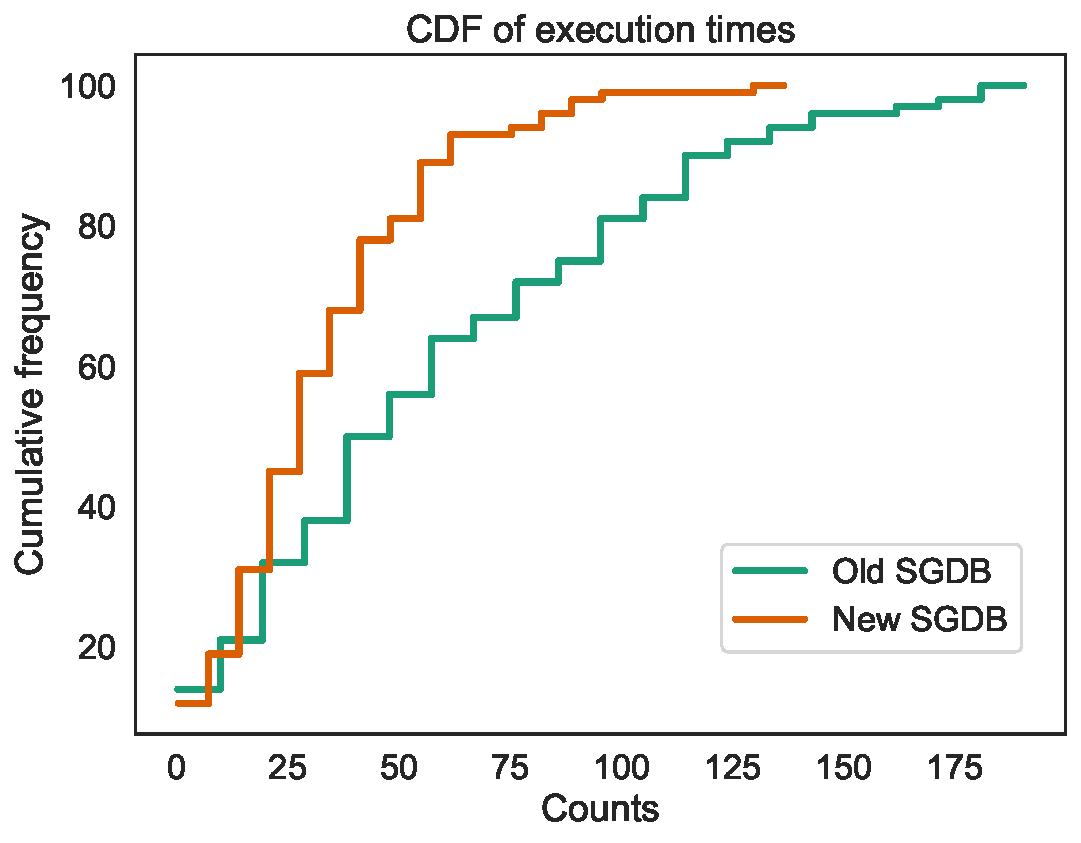
\includegraphics[width=0.6\textwidth]{../figs/extimes_CDF.pdf}
\caption{}\label{fig:cdf}
\end{figure}


\begin{figure} \centering
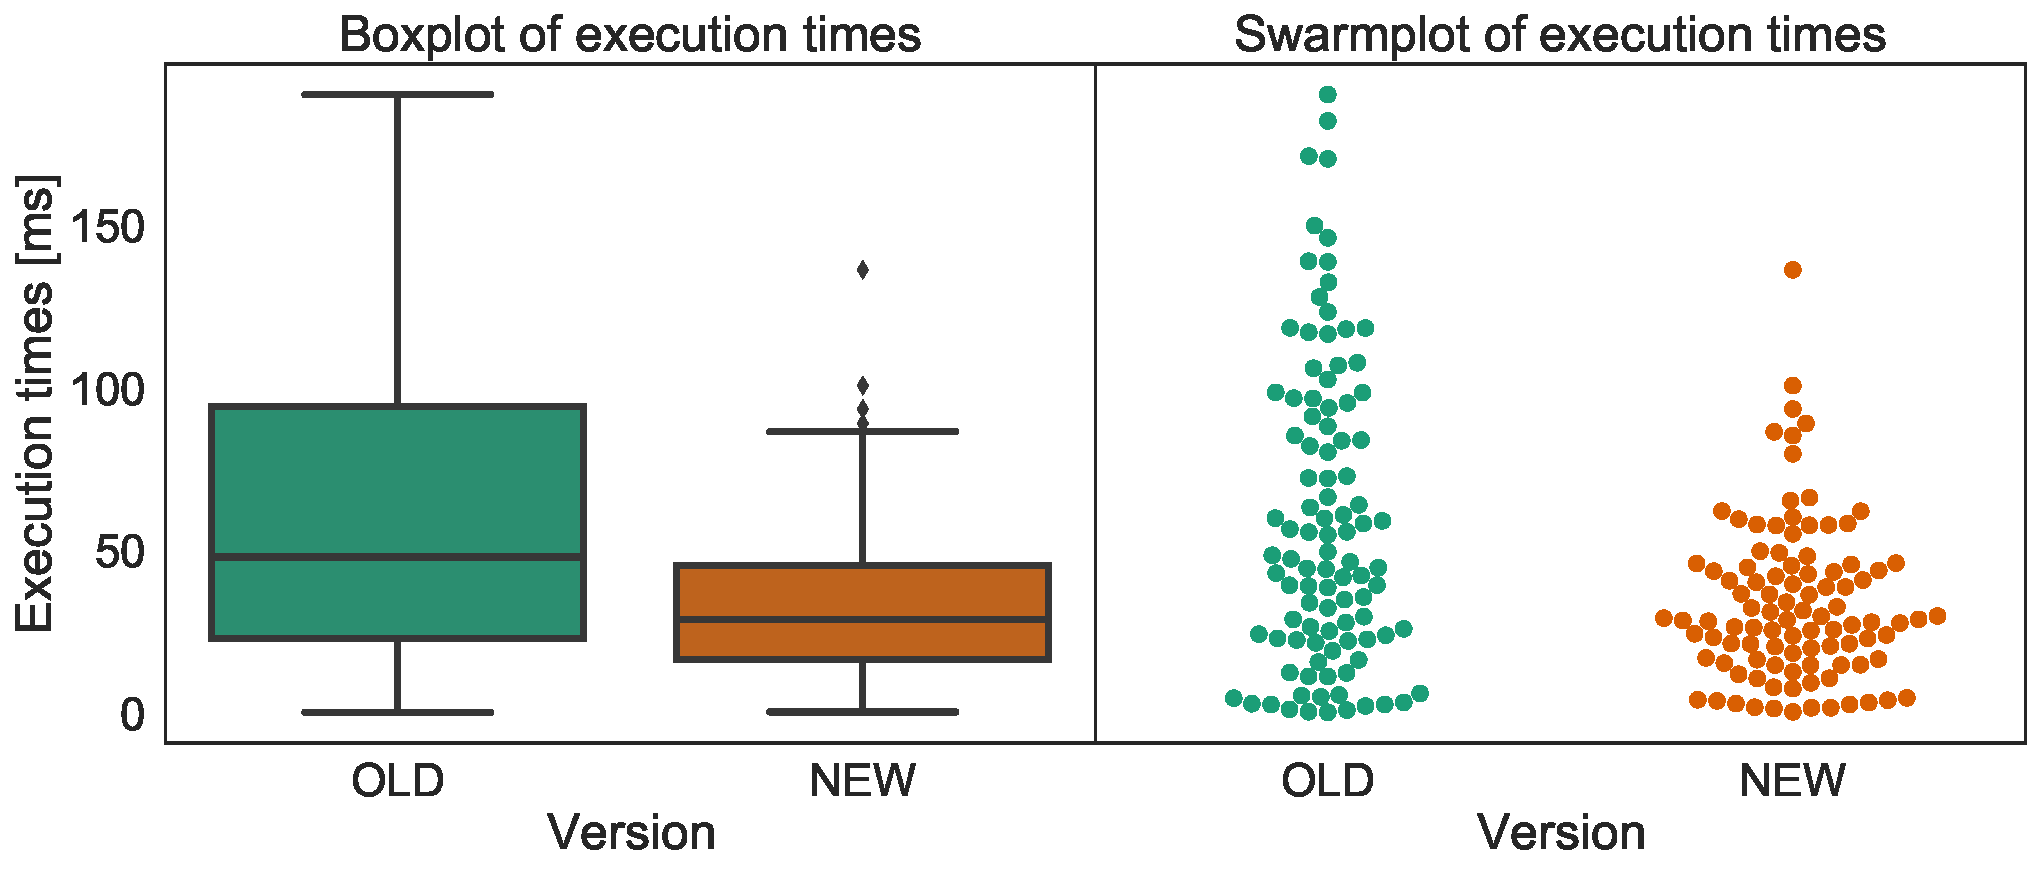
\includegraphics[width=0.9
\textwidth]{../figs/extimes_quantiles.pdf}
\caption{}\label{fig:boxswarm}
\end{figure}



\subsection{Confidence intervals}
Moreover, we could be interested in analyzing the improvement due to the new system. A possible way to quantify it consist of measuring the reduction in run time for the same sequence of tasks. In Figure \ref{fig:reduction}, the first panel shows the scatterplot of reductions in running time, the second exhibits the confidence intervals for the mean and for the median, while the right panel represents the distribution of reductions.
\begin{figure} \centering
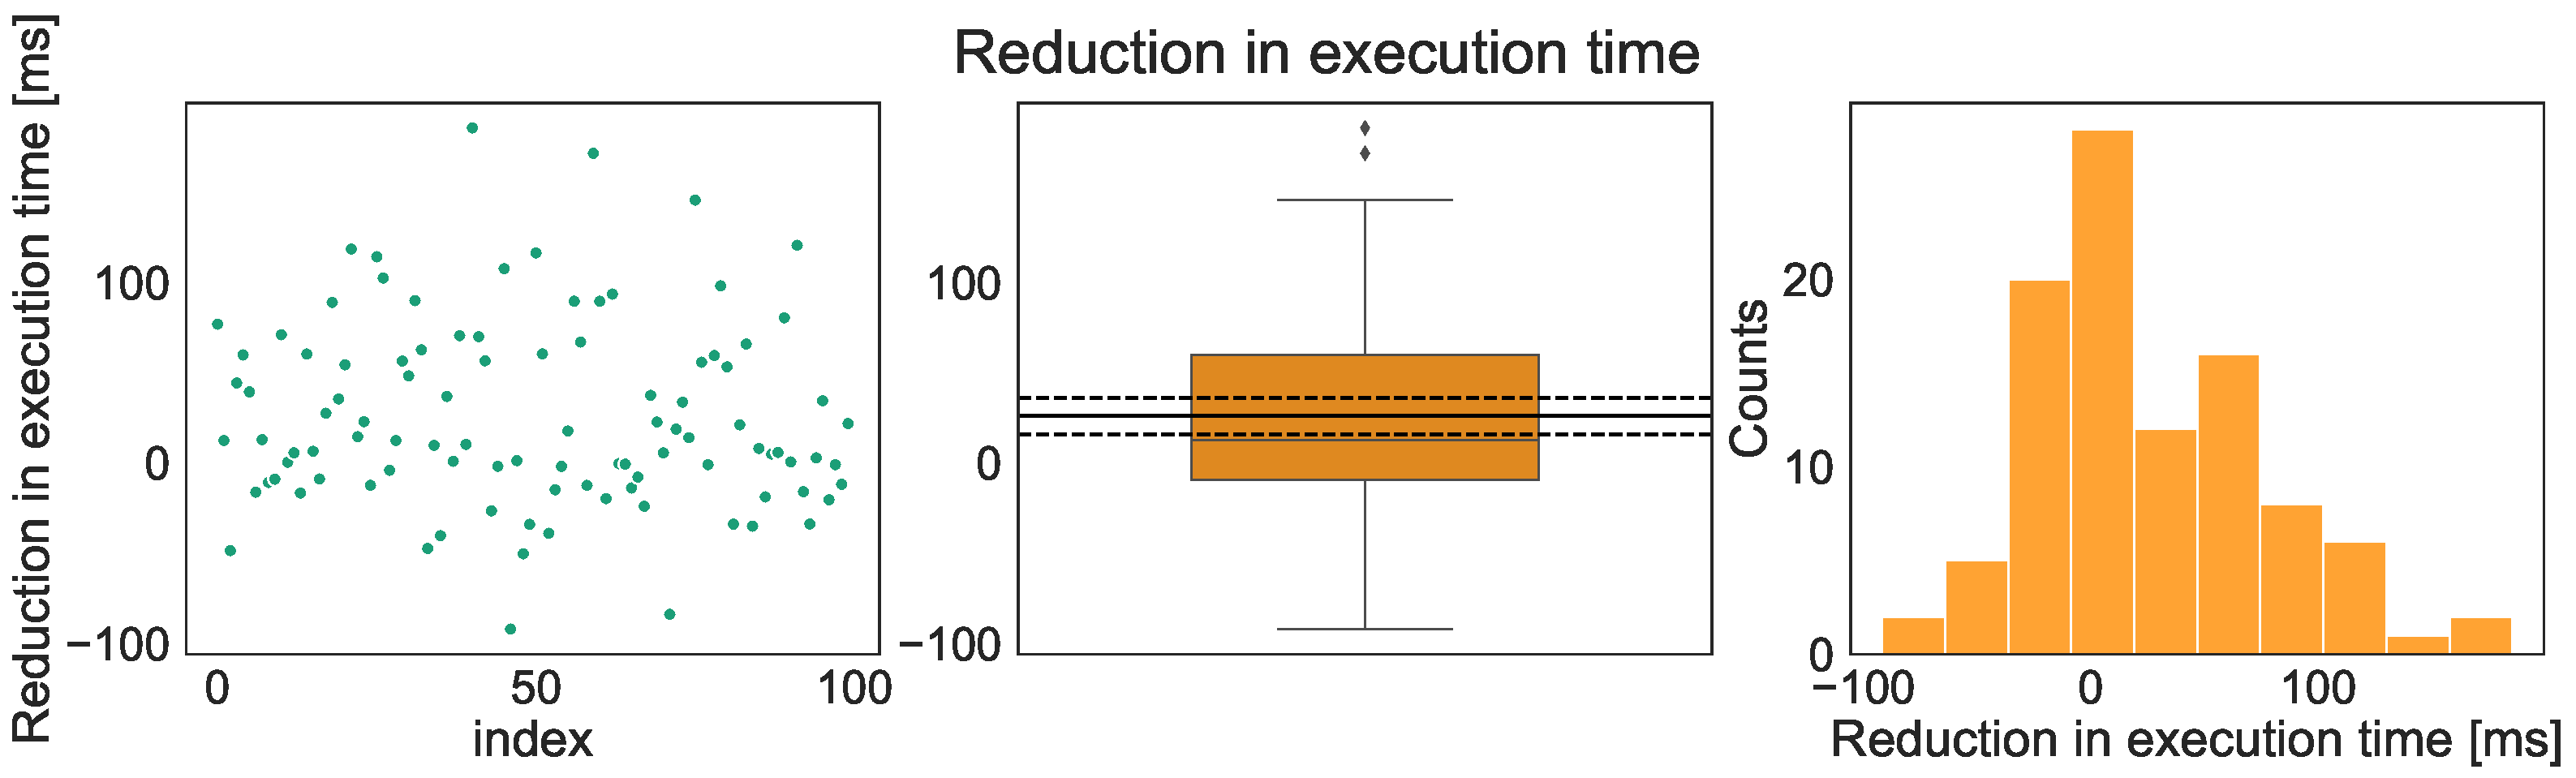
\includegraphics[width=1\textwidth]{../figs/extimes_reduction.pdf}
\caption{}\label{fig:reduction}
\end{figure}

From the theory we know different methods to compute confidence intervals for the mean. We already exploited the standard one to compute the CI of the run time reductions, but two more approaches can be investigated: once relies on the assumption that data are normally distributed, while the second consist of bootstrap method. In Figure \ref{fig:ci_methods} we show mean CI for all the methods proposed, both for the new and the old system.


\begin{figure} \centering
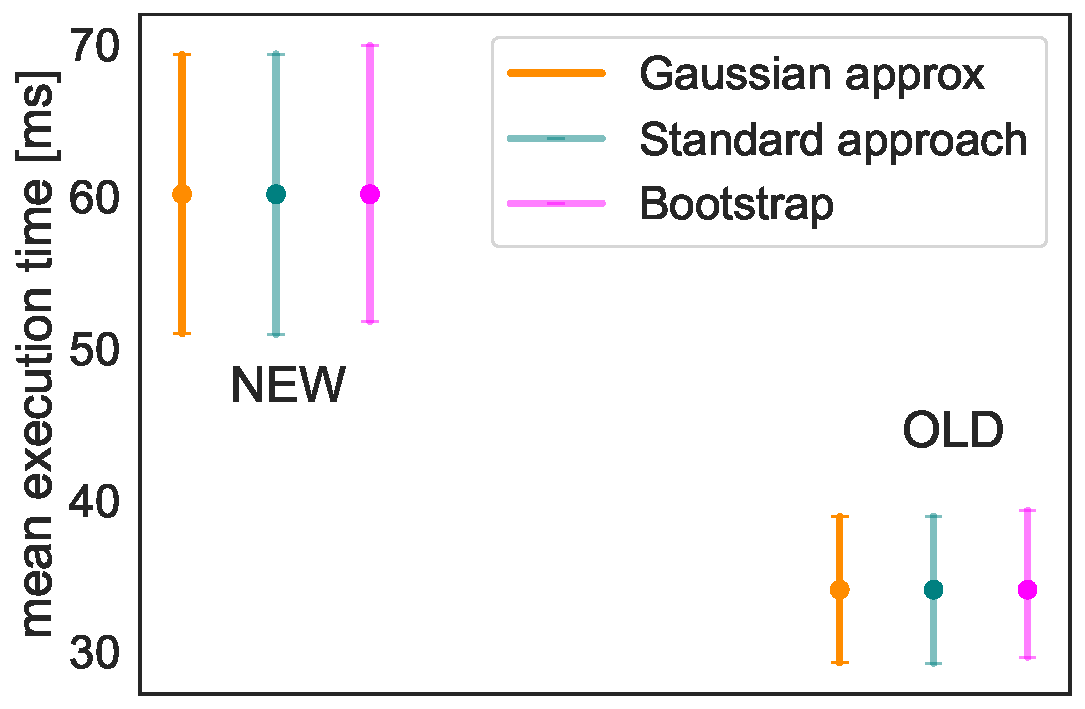
\includegraphics[width=0.6\textwidth]{../figs/CI_methods_comparison.pdf}
\caption{}\label{fig:ci_methods}
\end{figure}

All computations are carried out assuming a confidence level of 0.95.

\section{Simulation analysis}
In this section we perform a simulation, by means of Python Random Number Generators (RNG), to study the statistical properties of two distributions, uniform and normal, with particular reference to the computation of confidence intervals.

\subsection{Uniform distribution}
Let us consider $n$ iid data generated randomly and uniformly distributed: $x_i\sim \mathcal U ([0,1])$.

\subsubsection{Simulation with n=48}
mean: 0.55
std: 0.27
CI: [0.47, 0.62]

\subsubsection{Repetition of the experiment 1000 times}
Repeat the experiment independently for 1000 times
Observed probability of error 0.06.

\begin{figure} \centering
\begin{subfigure}{0.5\textwidth}
         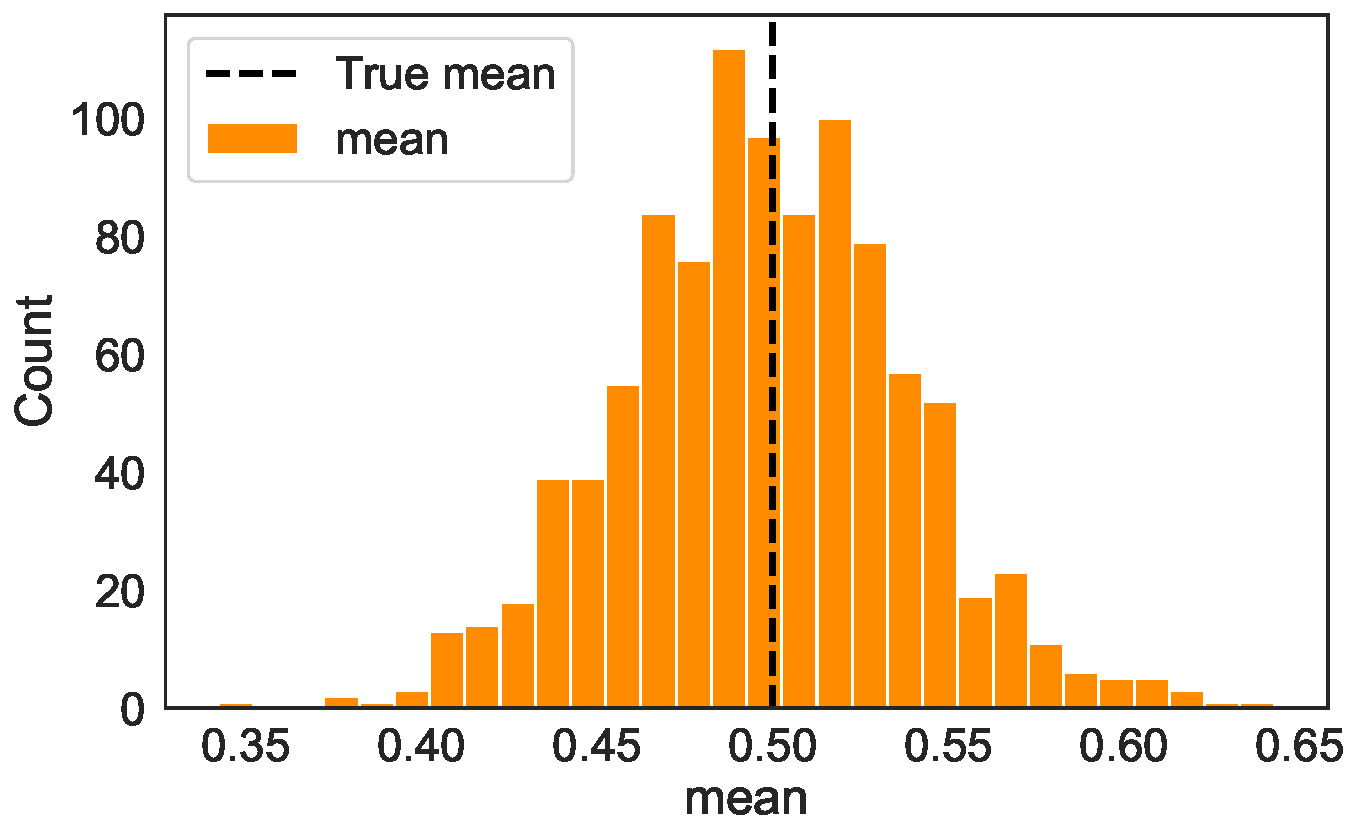
\includegraphics[width=\textwidth]{../figs/mean_distr_unif.pdf}
         \caption{$y=x$}\label{fig:y equals x}
     \end{subfigure}
     \begin{subfigure}{0.45\textwidth}
         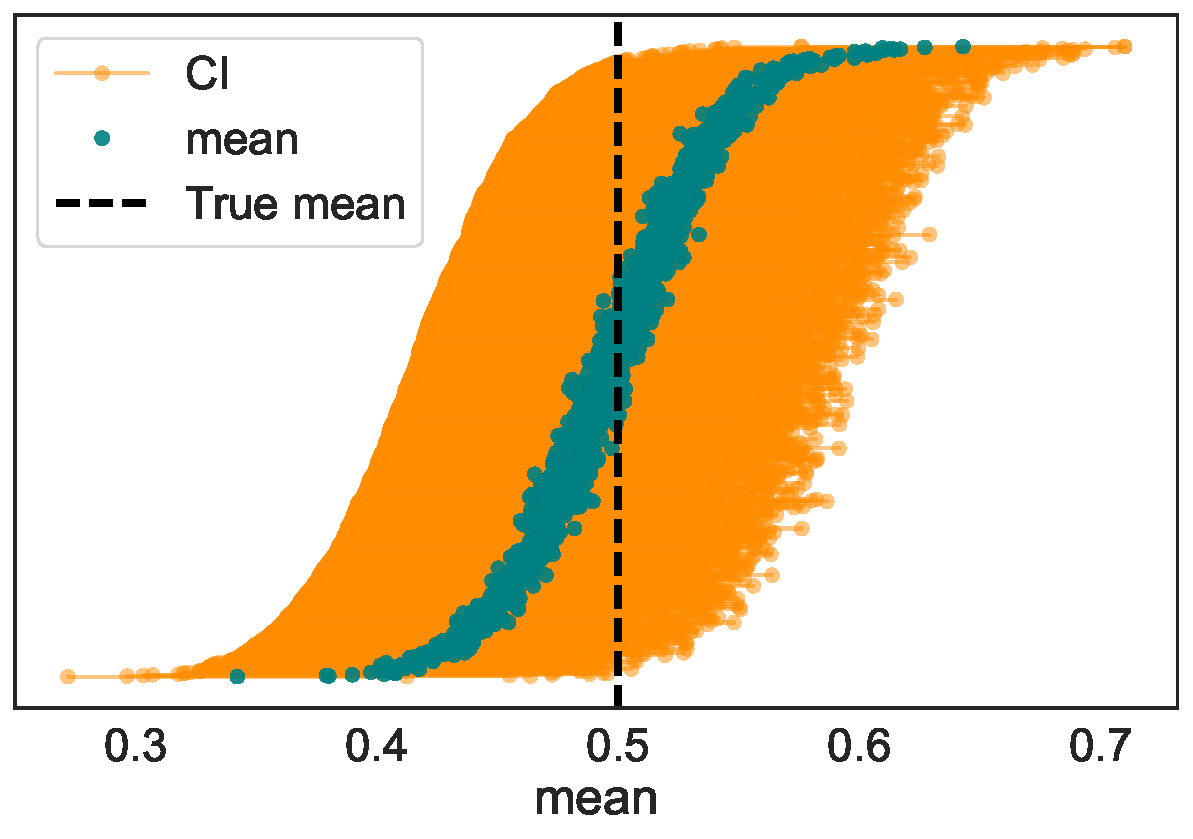
\includegraphics[width=\textwidth]{../figs/unif_mean_CI.pdf}
         \caption{$y=x$}
         \label{fig:y equals x}
     \end{subfigure}
    
  \caption{}\label{fig:ci_unif_mean}
\end{figure}



UNIFORM DISTRIBUTION


Repeat the experiment independently for 1000 times
Observed probability of error 0.06.

Simulation with n iid U(0,1) r.v.

Find confidence intervals for the VARIANCE vs. n
\begin{figure} \centering
\begin{subfigure}{0.45\textwidth}
         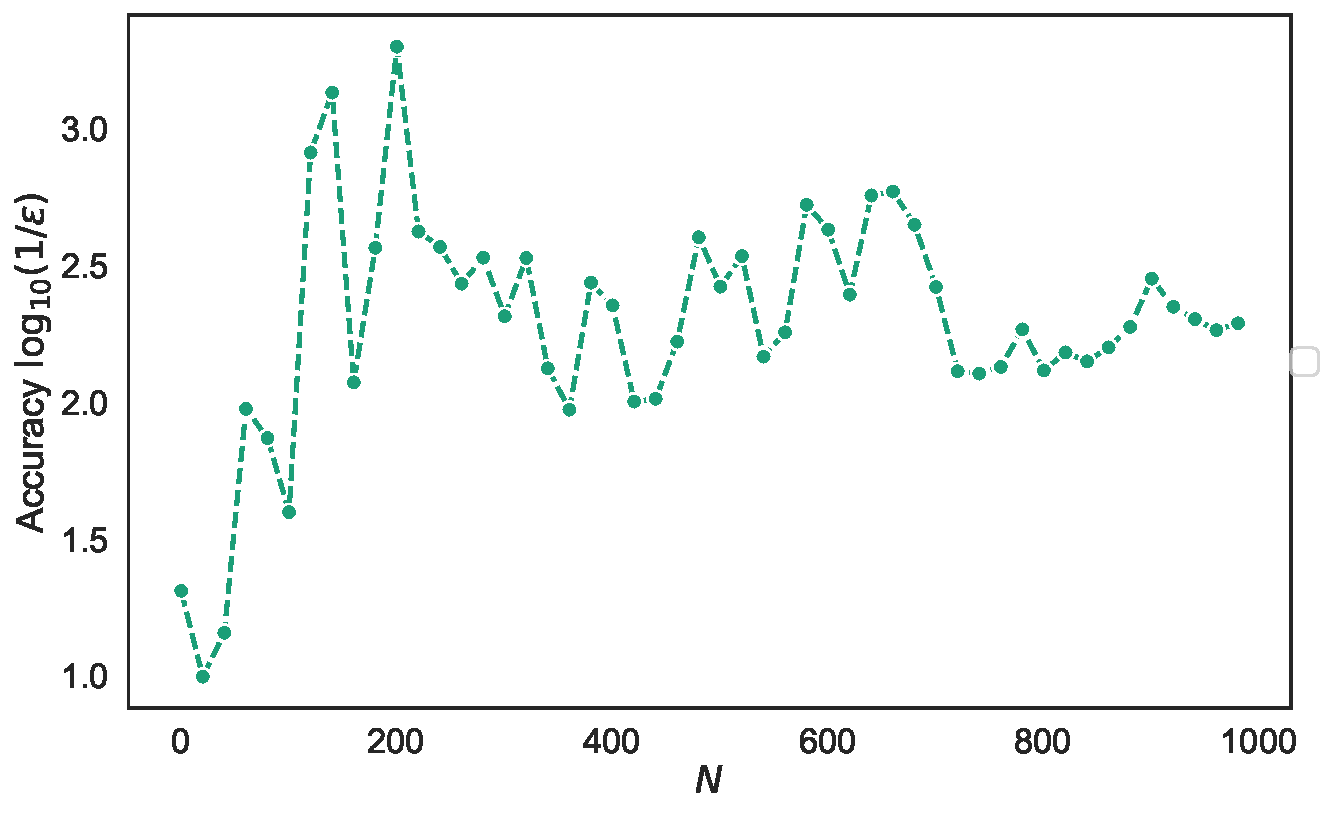
\includegraphics[width=\textwidth]{../figs/unif_mean_accuracy.pdf}
         \caption{$y=x$}\label{fig:y equals x}
     \end{subfigure}
     \begin{subfigure}{0.5\textwidth}
         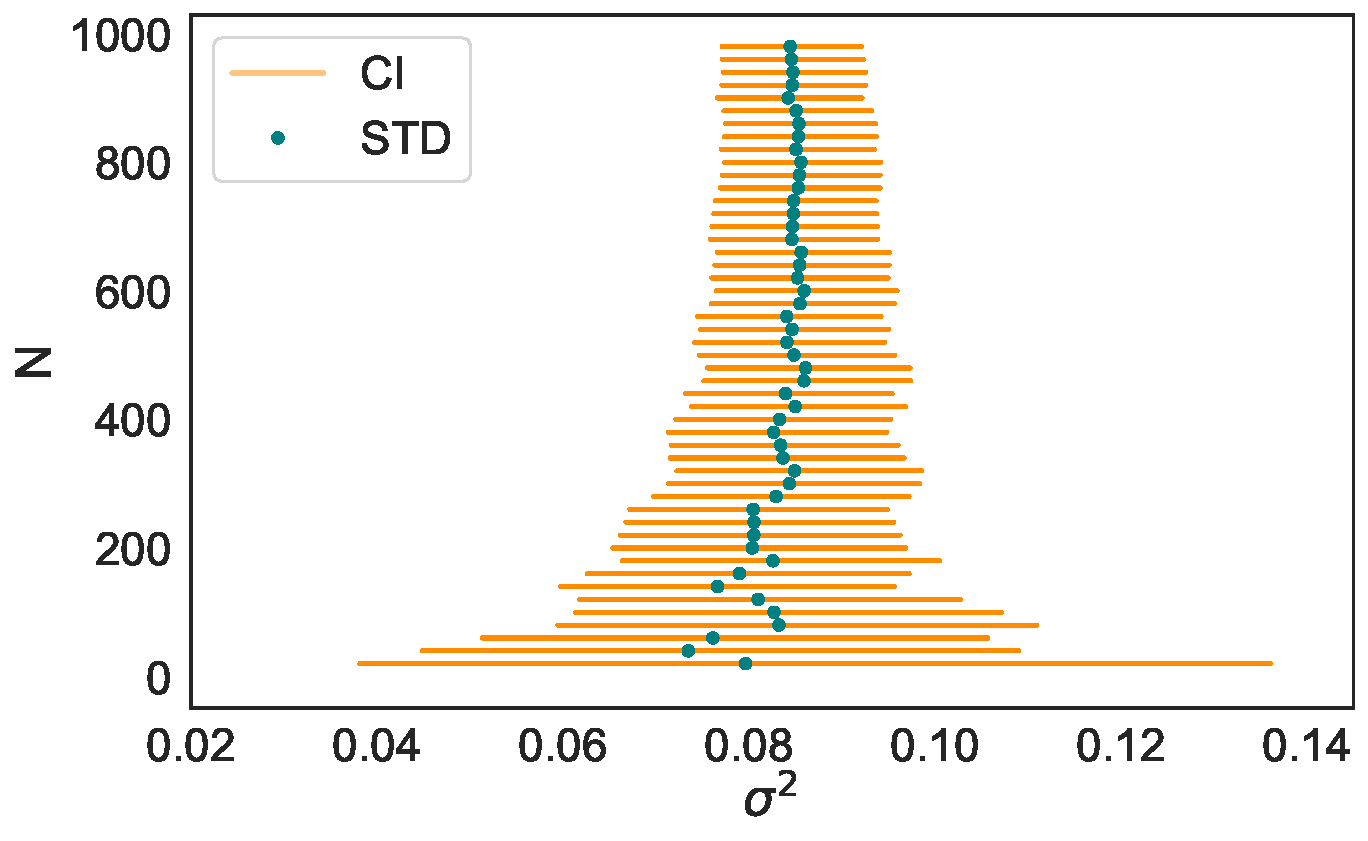
\includegraphics[width=\textwidth]{../figs/unif_variance_CI.pdf}
         \caption{$y=x$}
         \label{fig:y equals x}
     \end{subfigure}
  \caption{}\label{fig:N_unif}
\end{figure}

Find 95\% prediction interval using theory


NORMAL DISTRIBUTION
simulation with 48 iid norm(0,1)
mean: 0.18
std: 1.12
CI: [-0.13, 0.50]

Repeat the experiment independently for 1000 times
Observed probability of error 0.07.
\subsection{Normal distribution}
\begin{figure} \centering
\begin{subfigure}{0.5\textwidth}
         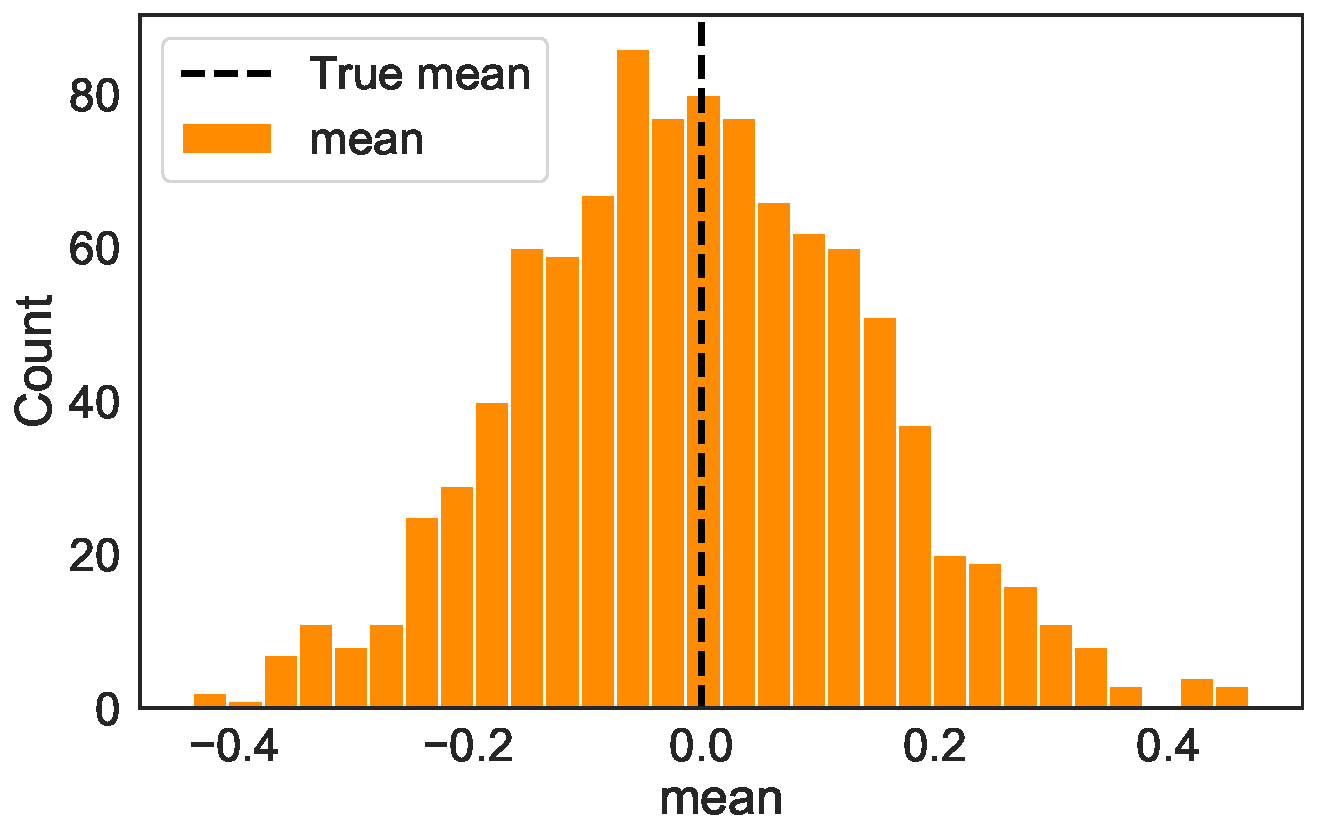
\includegraphics[width=\textwidth]{../figs/mean_distr_norm.pdf}
         \caption{$y=x$}\label{fig:y equals x}
     \end{subfigure}
     \begin{subfigure}{0.45\textwidth}
         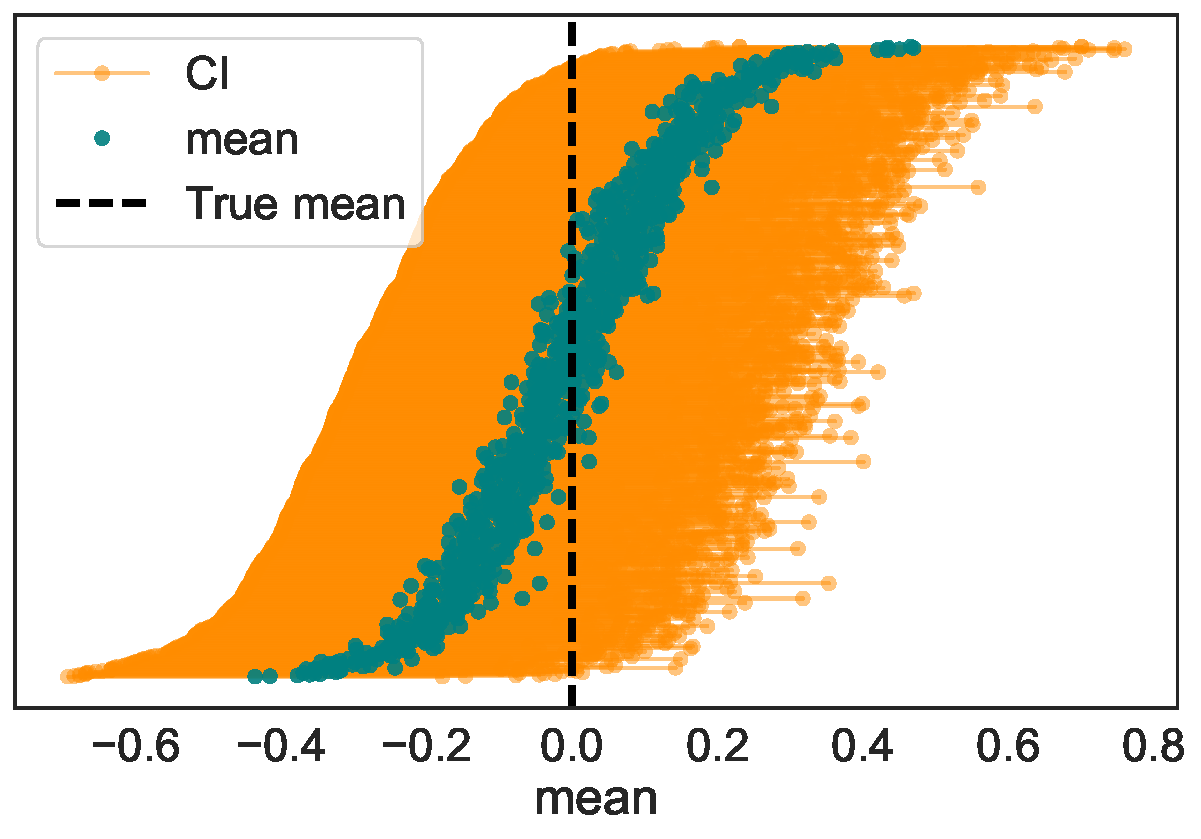
\includegraphics[width=\textwidth]{../figs/norm_mean_CI.pdf}
         \caption{$y=x$}
         \label{fig:y equals x}
     \end{subfigure}
  \caption{}\label{fig:ci_unif_mean}
\end{figure}

Simulation with n iid N(0,1) r.v.
Find confidence intervals for the variance vs. n
\begin{figure} \centering
\begin{subfigure}{0.45\textwidth}
         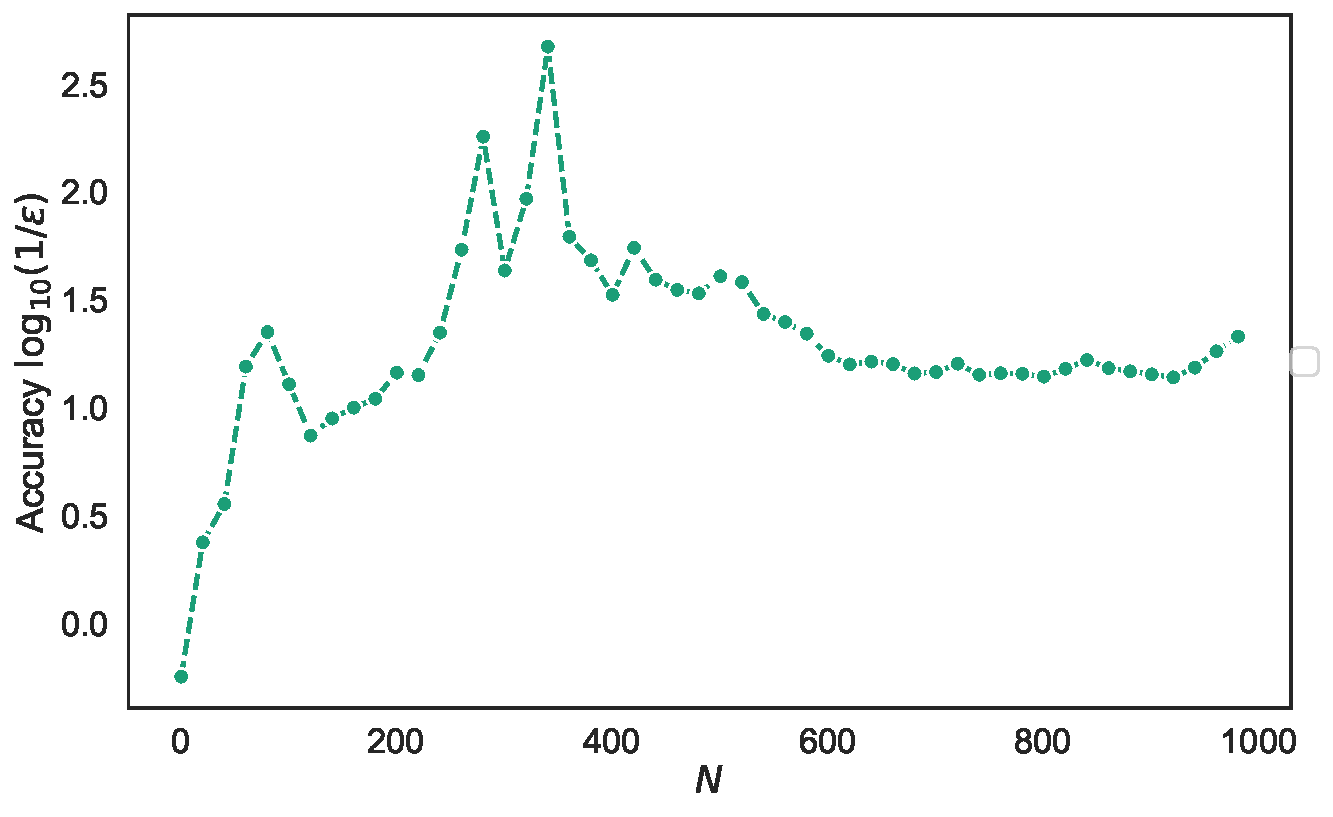
\includegraphics[width=\textwidth]{../figs/norm_mean_accuracy.pdf}
         \caption{$y=x$}\label{fig:y equals x}
     \end{subfigure}
     \begin{subfigure}{0.5\textwidth}
         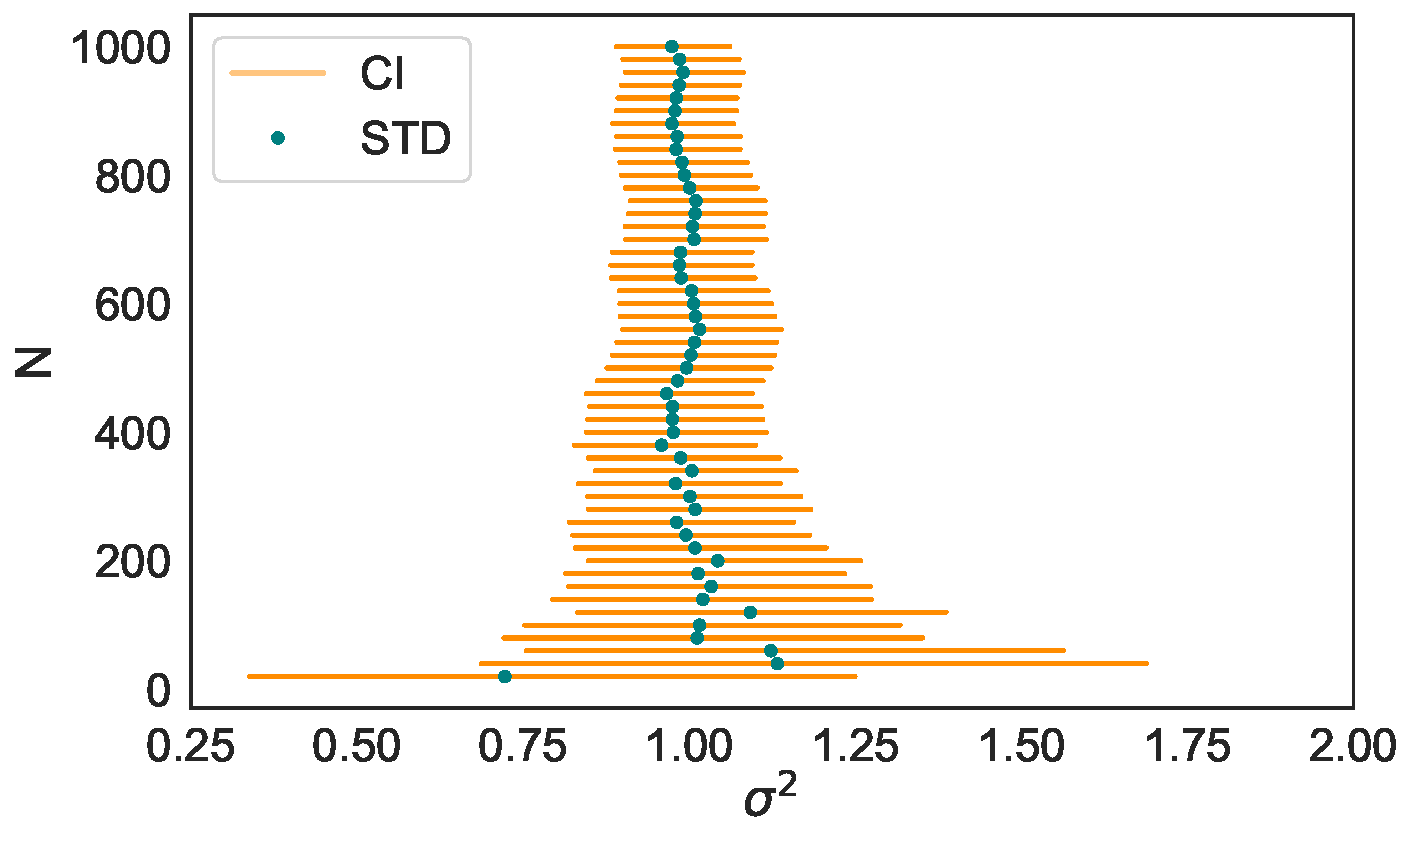
\includegraphics[width=\textwidth]{../figs/norm_variance_CI.pdf}
         \caption{$y=x$}
         \label{fig:y equals x}
     \end{subfigure}
  \caption{}\label{fig:N_unif}
\end{figure}




\end{document}
